\documentclass[10pt, aspectratio=169, handout]{beamer}
\usefonttheme{professionalfonts}
%\usetheme{CambridgeUS}
%
% Choose how your presentation looks.
%
% For more themes, color themes and font themes, see:
% http://deic.uab.es/~iblanes/beamer_gallery/index_by_theme.html
%
\mode<presentation>
{
  \usetheme{Berkeley}      % or try Darmstadt, Madrid, Warsaw, ...
  \usecolortheme{beaver} % or try albatross, beaver, crane, ...
  \usefonttheme{default}  % or try serif, structurebold, ...
  \setbeamertemplate{navigation symbols}{}
  \setbeamertemplate{caption}[numbered]
} 

\setbeamertemplate{footline}{%
  \leavevmode%
  \hbox{%
    \begin{beamercolorbox}[wd=.85\paperwidth,ht=2.5ex,dp=1ex,left]{author in head/foot}%
      \usebeamerfont{author in head/foot}Digital Signal Processing, Fall 2025%
    \end{beamercolorbox}%
    \begin{beamercolorbox}[wd=.15\paperwidth,ht=2.5ex,dp=1ex,right]{date in head/foot}%
      \hspace*{0.5em}\insertframenumber{} / \inserttotalframenumber\hspace*{0.5em}%
    \end{beamercolorbox}%
  }%
  \vskip0pt%
}

\usepackage[english]{babel}
\usepackage[utf8x]{inputenc}
\usepackage{tikz}
\usepackage{pgfplots}
\usepackage{array}  % for table column M
\usepackage{makecell} % to break line within a cell
\usepackage{verbatim}
\usepackage{graphicx}
\usepackage{subcaption}
\usepackage{amsfonts}
\usepackage{amsmath}
\usepackage{bm}
\usepackage{epstopdf}
\captionsetup{compatibility=false}
%\usepackage{dsfont}
\usepackage[absolute,overlay]{textpos}
\usetikzlibrary{calc}
\usetikzlibrary{pgfplots.fillbetween, backgrounds}
\usetikzlibrary{positioning}

\usetikzlibrary{pgfplots.groupplots}
\usetikzlibrary{plotmarks}
\usetikzlibrary{calc}

\usepgfplotslibrary{groupplots}
\pgfplotsset{compat=newest} 
%\pgfplotsset{plot coordinates/math parser=false}

\usepackage{ifthen}
\newboolean{showresults}
\setboolean{showresults}{false}

\usepackage{hyperref}
\hypersetup{
    colorlinks=true,
    linkcolor=blue,
    filecolor=magenta,      
    urlcolor=cyan,
}

% %% 
% \input{header.tex}

% %%
\title[ECEN 463/863]{Linear Constant-Coefficient Difference Equations}
\author{Maxx Seminario}
\institute{University of Nebraska-Lincoln}


\begin{document}
\begin{frame}
  \titlepage
\end{frame}

\section{Introduction}


\begin{frame}{Introduction to Difference Equations}
\begin{itemize}
    \item \textbf{Important Class of LTI Systems}: Systems where input $x[n]$ and output $y[n]$ satisfy a difference equation
    
    \item \textbf{General Form}:
    \[
        \sum_{k=0}^{N} a_k y[n-k] = \sum_{m=0}^{M} b_m x[n-m]
    \]
    
    \item \textbf{Parameters}:
    \begin{itemize}
        \item $N$: Order of the system (highest delay in output)
        \item $a_k$: Output coefficients (constant)
        \item $b_m$: Input coefficients (constant)
        \item $M$: Highest delay in input terms
    \end{itemize}
    
    \item \textbf{Why Important?}:
    \begin{itemize}
        \item Provides computational algorithms for LTI systems
        \item Foundation for digital filter implementation
        \item Connects time-domain and system analysis
    \end{itemize}
\end{itemize}
\end{frame}

\begin{frame}{Example 1: The Accumulator System}
    \textbf{Problem}: Find the difference equation for the accumulator system.

    % \vspace{0.3cm}
    \textbf{System Definition}:
    \[
        y[n] = \sum_{k=-\infty}^{n} x[k]
    \]

    % \vspace{0.3cm}
    \textbf{Approach}: 
    \begin{itemize}
        \item Rewrite the sum to separate current and past inputs
        \item Use the relationship between $y[n]$ and $y[n-1]$
    \end{itemize}
    \end{frame}

\section{Accumulator System}

\begin{frame}{Example 1: Accumulator Solution}
    \textbf{Step 1}: Rewrite the accumulator equation:
    \[
        y[n] = x[n] + \sum_{k=-\infty}^{n-1} x[k]
    \]

    % \vspace{0.3cm}
    \textbf{Step 2}: Recognize that the sum is $y[n-1]$:
    \[
        y[n-1] = \sum_{k=-\infty}^{n-1} x[k]
    \]

    % \vspace{0.3cm}
    \textbf{Step 3}: Substitute to get the difference equation:
    \[
        y[n] = x[n] + y[n-1]
    \]

    % \vspace{0.3cm}
    \textbf{Standard Form}:
    \[
        y[n] - y[n-1] = x[n]
    \]

    % \textbf{Parameters}: $N=1$, $a_0=1$, $a_1=-1$, $M=0$, $b_0=1$
\end{frame}

\begin{frame}{Block Diagram: Recursive Accumulator}
\begin{center}
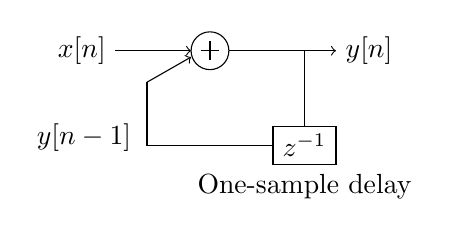
\begin{tikzpicture}[scale=0.8]
    % Input
    \draw[->] (-2, 0) -- (-0.8, 0);
    \node[left] at (-2, 0) {$x[n]$};
    
    % Summer - circle with plus
    \draw (-0.5, 0) circle (0.3);
    \draw (-0.65, 0) -- (-0.35, 0);
    \draw (-0.5, -0.15) -- (-0.5, 0.15);
    
    % Output line
    \draw[->] (-0.2, 0) -- (1.5, 0);
    \node[right] at (1.5, 0) {$y[n]$};
    
    % Feedback path
    \draw (1, 0) -- (1, -1.5) -- (-1.5, -1.5) -- (-1.5, -0.5);
    \draw[->] (-1.5, -0.5) -- (-0.8, -0.1);
    
    % Delay block (with white fill to cover lines underneath)
    \draw[fill=white] (0.5, -1.8) rectangle (1.5, -1.2);
    \node at (1, -1.5) {$z^{-1}$};
    \node[below] at (1, -1.8) {One-sample delay};
    
    % Feedback label
    \node[below] at (-2.5, -1) {$y[n-1]$};
\end{tikzpicture}
\end{center}

\vspace{0.3cm}
\textbf{Recursive Implementation}:
\begin{itemize}
    \item Each output value computed using previously computed values
    \item $y[n] = x[n] + y[n-1]$: Add current input to previous output
    \item Requires initial condition (e.g., $y[-1] = 0$)
\end{itemize}
\end{frame}

\section{Moving Average System}

\begin{frame}{Example 2: Moving Average System}
\textbf{Problem}: Find difference equation for causal moving average system.

\vspace{0.3cm}
\textbf{System Definition} (with $M_1 = 0$, so the system is causal):
\[
    y[n] = \frac{1}{M_2 + 1} \sum_{k=0}^{M_2} x[n-k]
\]

\vspace{0.3cm}
\textbf{Two Approaches}:
\begin{enumerate}
    \item \textbf{Direct (Non-recursive)}: Use convolution form directly
    \item \textbf{Recursive}: Express as cascade of simpler systems
\end{enumerate}
\end{frame}


\begin{frame}{Moving Average: Direct Implementation}
    \textbf{Direct Form}:
    \[
        y[n] = \frac{1}{M_2 + 1} \sum_{k=0}^{M_2} x[n-k]
    \]

    \vspace{0.3cm}
    \textbf{Standard Form}:
    \[
        y[n] = \sum_{k=0}^{M_2} \frac{1}{M_2 + 1} x[n-k]
    \]

    \vspace{0.3cm}

    \vspace{0.3cm}
    \textbf{Disadvantages of Direct Implementation}:
    \begin{itemize}
        \item Requires $(M_2 + 1)$ multiplications per output sample
        \item Must store $(M_2 + 1)$ input samples in memory
        \item $O(M_2)$ : Computational cost grows linearly with window size $M_2$
    \end{itemize}
\end{frame}




\begin{frame}{Block Diagram: Recursive Moving Average}
\begin{center}
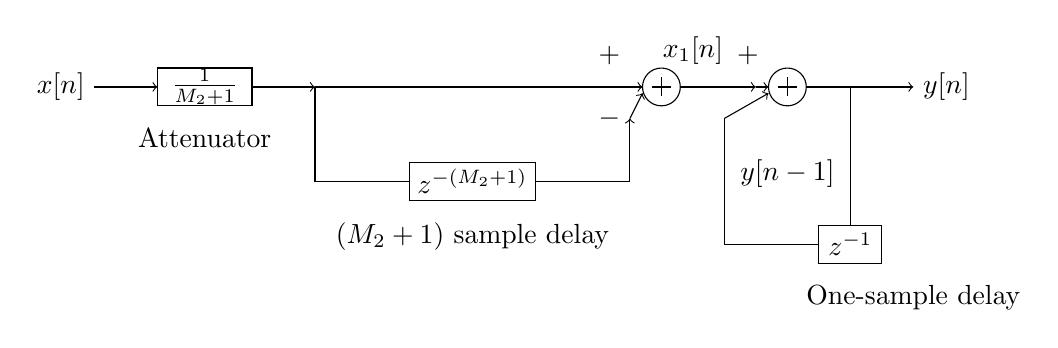
\begin{tikzpicture}[scale=0.8]
    % Input
    \draw[->] (-3, 0) -- (-2, 0);
    \node[left] at (-3, 0) {$x[n]$};
    
    % Attenuator
    \draw[fill=white] (-2, -0.3) rectangle (-0.5, 0.3);
    \node at (-1.25, 0) {$\frac{1}{M_2+1}$};
    \node[below] at (-1.25, -0.5) {Attenuator};
    
    % Output of attenuator
    \draw[->] (-0.5, 0) -- (0.5, 0);
    
    % Split path for delay
    \draw (0.5, 0) -- (0.5, -1.5) -- (2, -1.5);
    
    % M2+1 sample delay
    \draw[fill=white] (2, -1.8) rectangle (4, -1.2);
    \node at (3, -1.5) {$z^{-(M_2+1)}$};
    \node[below] at (3, -2) {$(M_2+1)$ sample delay};
    
    % Output of delay
    \draw[->] (4, -1.5) -- (5.5, -1.5) -- (5.5, -0.5);
    
    % Summer for x1[n] (circle with plus and minus)
    \draw (6, 0) circle (0.3);
    \draw (5.85, 0) -- (6.15, 0);
    \draw (6, -0.15) -- (6, 0.15);
    \node[above left] at (5.5, 0.2) {$+$};
    \node[below left] at (5.5, -0.2) {$-$};
    
    % Direct path to summer
    \draw[->] (0.5, 0) -- (5.7, 0);
    
    % Delay path to summer
    \draw[->] (5.5, -0.5) -- (5.7, -0.1);
    
    % Output of first summer (x1[n])
    \draw[->] (6.3, 0) -- (7.5, 0);
    \node[above] at (6.5, 0.2) {$x_1[n]$};
    
    % Accumulator summer (circle with plus)
    \draw (8, 0) circle (0.3);
    \draw (7.85, 0) -- (8.15, 0);
    \draw (8, -0.15) -- (8, 0.15);
    \node[above left] at (7.7, 0.2) {$+$};
    
    % Input to accumulator
    \draw[->] (7.5, 0) -- (7.7, 0);
    
    % Output
    \draw[->] (8.3, 0) -- (10, 0);
    \node[right] at (10, 0) {$y[n]$};
    
    % Feedback path for accumulator
    \draw (9, 0) -- (9, -2.5) -- (7, -2.5) -- (7, -0.5);
    \draw[->] (7, -0.5) -- (7.7, -0.1);
    
    % Delay in feedback path
    \draw[fill=white] (8.5, -2.8) rectangle (9.5, -2.2);
    \node at (9, -2.5) {$z^{-1}$};
    \node[below] at (10, -3) {One-sample delay};
    
    % Feedback label
    \node[below] at (8, -1) {$y[n-1]$};
    
    % Label for delayed input
    % \node[right] at (6, 0) {$x[n-(M_2+1)]$};
    
\end{tikzpicture}
\end{center}

\vspace{0.3cm}
\textbf{Signal Flow}:
\begin{itemize}
    \item Input $x[n]$ → Attenuator $\frac{1}{M_2+1}$ 
    \item Attenuated signal splits: direct path and $(M_2+1)$ sample delay
    \item Sum: $x_1[n] = \frac{1}{M_2+1}[x[n] - x[n-(M_2+1)]]$
    \item $x_1[n]$ → Accumulator → Output $y[n]$
\end{itemize}
\end{frame}






\begin{frame}{Moving Average as Difference Equation}

    \vspace{0.3cm}
    \textbf{Intermediate signal}:
    \[
        x_1[n] = \frac{1}{M_2 + 1}[x[n] - x[n - M_2 - 1]]
    \]

    \vspace{0.3cm}
    \textbf{Accumulator relation}: $y[n] = x_1[n] + y[n-1]$

    \vspace{0.3cm}
    \textbf{Final recursive form}:
    \[
        y[n] - y[n-1] = \frac{1}{M_2 + 1}[x[n] - x[n - M_2 - 1]]
    \]

    Note: There is an unlimited number of distinct difference equations to represent an LTI I/O relation.

\end{frame}

\section{General Solution}

\begin{frame}{General Solution of Difference Equations}
    \textbf{Key Issue}: Difference equation alone does not uniquely specify output!

    \vspace{0.3cm}
    \textbf{General Solution Structure}:
    \[
        y[n] = y_p[n] + y_h[n]
    \]

    \begin{itemize}
        \item $y_p[n]$: Particular solution (satisfies original equation)
        \item $y_h[n]$: Homogeneous solution (satisfies homogeneous equation)
    \end{itemize}

    % \vspace{0.3cm}
    \textbf{Homogeneous Equation (x[n] = 0)}:
    \[
        \sum_{k=0}^{N} a_k y_h[n-k] = 0
    \]

    % \vspace{0.3cm}
    \textbf{Homogeneous Solution Form}:
    \[
        y_h[n] = \sum_{m=1}^{N} A_m z_m^n
    \]
    where $z_m$ are roots of characteristic polynomial $A(z) = \sum_{k=0}^{N} a_k z^{-k} = 0$
\end{frame}

\section{Particular Solution}

\begin{frame}{Auxiliary Conditions}
    \textbf{Need for Auxiliary Conditions}:
    \begin{itemize}
        \item $N$ undetermined coefficients $A_m$ in homogeneous solution
        \item Need $N$ auxiliary (boundary) conditions for unique solution
    \end{itemize}

    % \vspace{0.3cm}
    \textbf{Types of Auxiliary Conditions}:
    \begin{enumerate}
        \item \textbf{Fixed Values}: Specify $y[-1], y[-2], \ldots, y[-N]$
        \item \textbf{Initial Rest}: If $x[n] = 0$ for $n < n_0$, then $y[n] = 0$ for $n < n_0$
    \end{enumerate}
\end{frame}

\begin{frame}{Forward and Backward Computation for Specific Class of Difference Equations}
    \textbf{Specific Class of Difference Equations}:
    \begin{itemize}
        \item Inputs $x[n]$ and Outputs $y[n]$ satisfy an $N$th-order linear constant coefficient difference equation:
        \[
            \sum_{k=0}^N a_k y[n-k] = \sum_{k=0}^M b_k x[n-k]
        \]
        \[
            a_0 y[n] + a_1 y[n-1] + \cdots + a_N y[n-N] = b_0 x[n] + b_1 x[n-1] + \cdots + b_M x[n-M]
        \]
    \end{itemize}

    % \vspace{0.3cm}
    \textbf{Recursive Computation} (forward):
    \[
        y[n] = -\sum_{k=1}^{N} \frac{a_k}{a_0} y[n-k] + \sum_{k=0}^{M} \frac{b_k}{a_0} x[n-k]
    \]

    % \vspace{0.3cm}
    \textbf{Recursive Computation} (backward):
    \[
        y[n-N] = -\sum_{k=0}^{N-1} \frac{a_k}{a_N} y[n-k] + \sum_{k=0}^{M} \frac{b_k}{a_N} x[n-k]
    \]
\end{frame}


\begin{frame}{Example 3: First-Order Difference Equation}
\textbf{Problem}: Solve the difference equation with given input and initial condition.

\vspace{0.3cm}
\textbf{Difference Equation}:
\[
    y[n] = ay[n-1] + x[n]
\]

\vspace{0.3cm}
\textbf{Input}:
\[
    x[n] = K\delta[n]
\]

\vspace{0.3cm}
\textbf{Auxiliary Condition}:
\[
    y[-1] = c
\]

\vspace{0.3cm}
\textbf{Find}: The complete solution $y[n]$ for all $n$.
\end{frame}


\ifthenelse{\boolean{showresults}}{
\begin{frame}{Example 3: Solution for $n > 0$}
\textbf{Method}: Use recursive computation starting from $n = 0$.

\vspace{0.3cm}
\textbf{For $n = 0$}:
\begin{align}
    y[0] &= ay[-1] + x[0] \\
    &= ay[-1] + K\delta[0] \\
    &= ac + K \cdot 1 \\
    &= ac + K
\end{align}

\vspace{0.3cm}
\textbf{For $n = 1$}:
\begin{align}
    y[1] &= ay[0] + x[1] \\
    &= a(ac + K) + K\delta[1] \\
    &= a^2c + aK + K \cdot 0 \\
    &= a^2c + aK
\end{align}
\end{frame}

\begin{frame}{Example 3: Solution for $n > 0$}
\textbf{For $n = 2$}:
\begin{align}
    y[2] &= ay[1] + x[2] \\
    &= a(a^2c + aK) + K\delta[2] \\
    &= a^3c + a^2K + 0 \\
    &= a^3c + a^2K
\end{align}

\vspace{0.3cm}
\textbf{For $n = 3$}:
\begin{align}
    y[3] &= ay[2] + x[3] \\
    &= a(a^3c + a^2K) + 0 \\
    &= a^4c + a^3K
\end{align}

\vspace{0.3cm}
\textbf{Pattern Recognition}:
For $n \geq 0$: $y[n] = a^{n+1}c + a^nK$
\end{frame}


\begin{frame}{Example 3: Solution for $n < 0$}
    \textbf{For $n < 0$}: Use backward recursion.

    % \vspace{0.3cm}
    \textbf{Rearrange difference equation}:
    \[
        y[n-1] = \frac{y[n] - x[n]}{a}
    \]

    % \vspace{0.3cm}
    \textbf{For $n = 0$ (find $y[-1]$)}:
    \[
        y[-1] = \frac{y[0] - x[0]}{a} = \frac{(ac + K) - K}{a} = \frac{ac}{a} = c
    \]
    This confirms our auxiliary condition 

    % \vspace{0.3cm}
    \textbf{For $n = -1$ (find $y[-2]$)}:
    \[
        y[-2] = \frac{y[-1] - x[-1]}{a} = \frac{c - 0}{a} = \frac{c}{a}
    \]

    % \vspace{0.3cm}
    \textbf{General pattern for $n < 0$}:
    \[
        y[n] = ca^{n+1} = \frac{c}{a^{n+1}}
    \]
\end{frame}

\begin{frame}{Example 3: Complete Solution}
\textbf{Final Answer}:
\[
    y[n] = \begin{cases}
        ca^{n+1}, & n < 0 \\
        a^n(ac + K), & n \geq 0
    \end{cases}
\]

\vspace{0.3cm}
\textbf{Alternative Compact Form}:
\[
    y[n] = ca^{n+1} + Ka^n u[n]
\]
where $u[n]$ is the unit step function.

\vspace{0.3cm}
\textbf{Physical Interpretation}:
\begin{itemize}
    \item \textbf{Homogeneous part}: $ca^{n+1}$ (due to initial condition)
    \item \textbf{Forced response}: $Ka^n u[n]$ (due to impulse input)
    \item \textbf{System behavior}: Exponential with base $a$
    \item \textbf{Stability}: System stable if $|a| < 1$
\end{itemize}
\end{frame}
}{}

\section{Summary}

\begin{frame}{Summary: Linear Constant-Coefficient Difference Equations}
    \begin{itemize}
        \item \textbf{Definition}:
        \[
            \sum_{k=0}^N a_k y[n-k] = \sum_{m=0}^M b_m x[n-m]
        \]
        Describes the relationship between input $x[n]$ and output $y[n]$ in LTI systems.

        \item \textbf{Key Components}:
        \begin{itemize}
            \item $N$ and $M$: Order of the system
            \item $a_k, b_m$: Constant coefficients
            \item Recursive and direct computation methods
        \end{itemize}

        \item \textbf{General Solution}:
        \[
            y[n] = y_p[n] + y_h[n]
        \]
        \begin{itemize}
            \item $y_p[n]$: Particular solution (due to input $x[n]$)
            \item $y_h[n]$: Homogeneous solution (due to initial conditions)
            \item Auxiliary conditions: Necessary to determine a unique / particular solutions.
        \end{itemize}


        \item \textbf{Applications}: Digital filters, computational algorithms for LTI systems, and time-domain analysis.
    \end{itemize}
\end{frame}



\end{document}
